\documentclass{standalone}
\usepackage{tikz}
\begin{document}

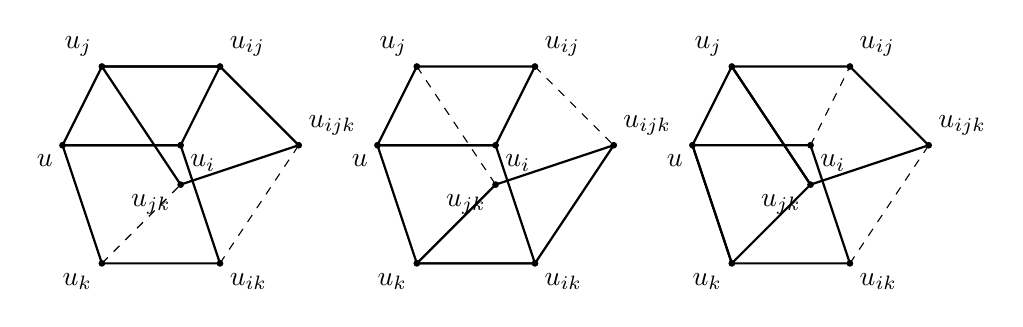
\begin{tikzpicture}

% Cube 1
\begin{scope}
    \coordinate (u) at (0,0);
    \coordinate (ui) at (1.5,0);
    \coordinate (uj) at (0.5,1);
    \coordinate (uij) at (2,1);
    \coordinate (uk) at (0.5,-1.5);
    \coordinate (uik) at (2,-1.5);
    \coordinate (ujk) at (1.5,-0.5);
    \coordinate (uijk) at (3,0);

    \draw[thick] (u) -- (ui) -- (uij) -- (uj) -- cycle;
    \draw[thick] (u) -- (uk) -- (uik) -- (ui) -- cycle;
    \draw[thick] (uj) -- (ujk) -- (uijk) -- (uij) -- cycle;
    \draw[dashed] (uk) -- (ujk);
    \draw[dashed] (uik) -- (uijk);

    \filldraw (u) circle (1pt) node[below left] {$u$};
    \filldraw (ui) circle (1pt) node[below right] {$u_i$};
    \filldraw (uj) circle (1pt) node[above left] {$u_j$};
    \filldraw (uij) circle (1pt) node[above right] {$u_{ij}$};
    \filldraw (uk) circle (1pt) node[below left] {$u_k$};
    \filldraw (uik) circle (1pt) node[below right] {$u_{ik}$};
    \filldraw (ujk) circle (1pt) node[below left] {$u_{jk}$};
    \filldraw (uijk) circle (1pt) node[above right] {$u_{ijk}$};
\end{scope}

% Cube 2
\begin{scope}[xshift=4cm]
    \coordinate (u) at (0,0);
    \coordinate (ui) at (1.5,0);
    \coordinate (uj) at (0.5,1);
    \coordinate (uij) at (2,1);
    \coordinate (uk) at (0.5,-1.5);
    \coordinate (uik) at (2,-1.5);
    \coordinate (ujk) at (1.5,-0.5);
    \coordinate (uijk) at (3,0);

    \draw[thick] (u) -- (ui) -- (uik) -- (uk) -- cycle;
    \draw[thick] (u) -- (uj) -- (uij) -- (ui) -- cycle;
    \draw[thick] (uk) -- (ujk) -- (uijk) -- (uik) -- cycle;
    \draw[dashed] (uj) -- (ujk);
    \draw[dashed] (uij) -- (uijk);

    \filldraw (u) circle (1pt) node[below left] {$u$};
    \filldraw (ui) circle (1pt) node[below right] {$u_i$};
    \filldraw (uj) circle (1pt) node[above left] {$u_j$};
    \filldraw (uij) circle (1pt) node[above right] {$u_{ij}$};
    \filldraw (uk) circle (1pt) node[below left] {$u_k$};
    \filldraw (uik) circle (1pt) node[below right] {$u_{ik}$};
    \filldraw (ujk) circle (1pt) node[below left] {$u_{jk}$};
    \filldraw (uijk) circle (1pt) node[above right] {$u_{ijk}$};
\end{scope}

% Cube 3
\begin{scope}[xshift=8cm]
    \coordinate (u) at (0,0);
    \coordinate (ui) at (1.5,0);
    \coordinate (uj) at (0.5,1);
    \coordinate (uij) at (2,1);
    \coordinate (uk) at (0.5,-1.5);
    \coordinate (uik) at (2,-1.5);
    \coordinate (ujk) at (1.5,-0.5);
    \coordinate (uijk) at (3,0);

    \draw[thick] (u) -- (uj) -- (ujk) -- (uk) -- cycle;
    \draw[thick] (u) -- (ui) -- (uik) -- (uk) -- cycle;
    \draw[thick] (uj) -- (uij) -- (uijk) -- (ujk) -- cycle;
    \draw[dashed] (ui) -- (uij);
    \draw[dashed] (uik) -- (uijk);

    \filldraw (u) circle (1pt) node[below left] {$u$};
    \filldraw (ui) circle (1pt) node[below right] {$u_i$};
    \filldraw (uj) circle (1pt) node[above left] {$u_j$};
    \filldraw (uij) circle (1pt) node[above right] {$u_{ij}$};
    \filldraw (uk) circle (1pt) node[below left] {$u_k$};
    \filldraw (uik) circle (1pt) node[below right] {$u_{ik}$};
    \filldraw (ujk) circle (1pt) node[below left] {$u_{jk}$};
    \filldraw (uijk) circle (1pt) node[above right] {$u_{ijk}$};
\end{scope}

\end{tikzpicture}

\end{document}